


\tikzset{every picture/.style={line width=0.75pt}} %set default line width to 0.75pt        

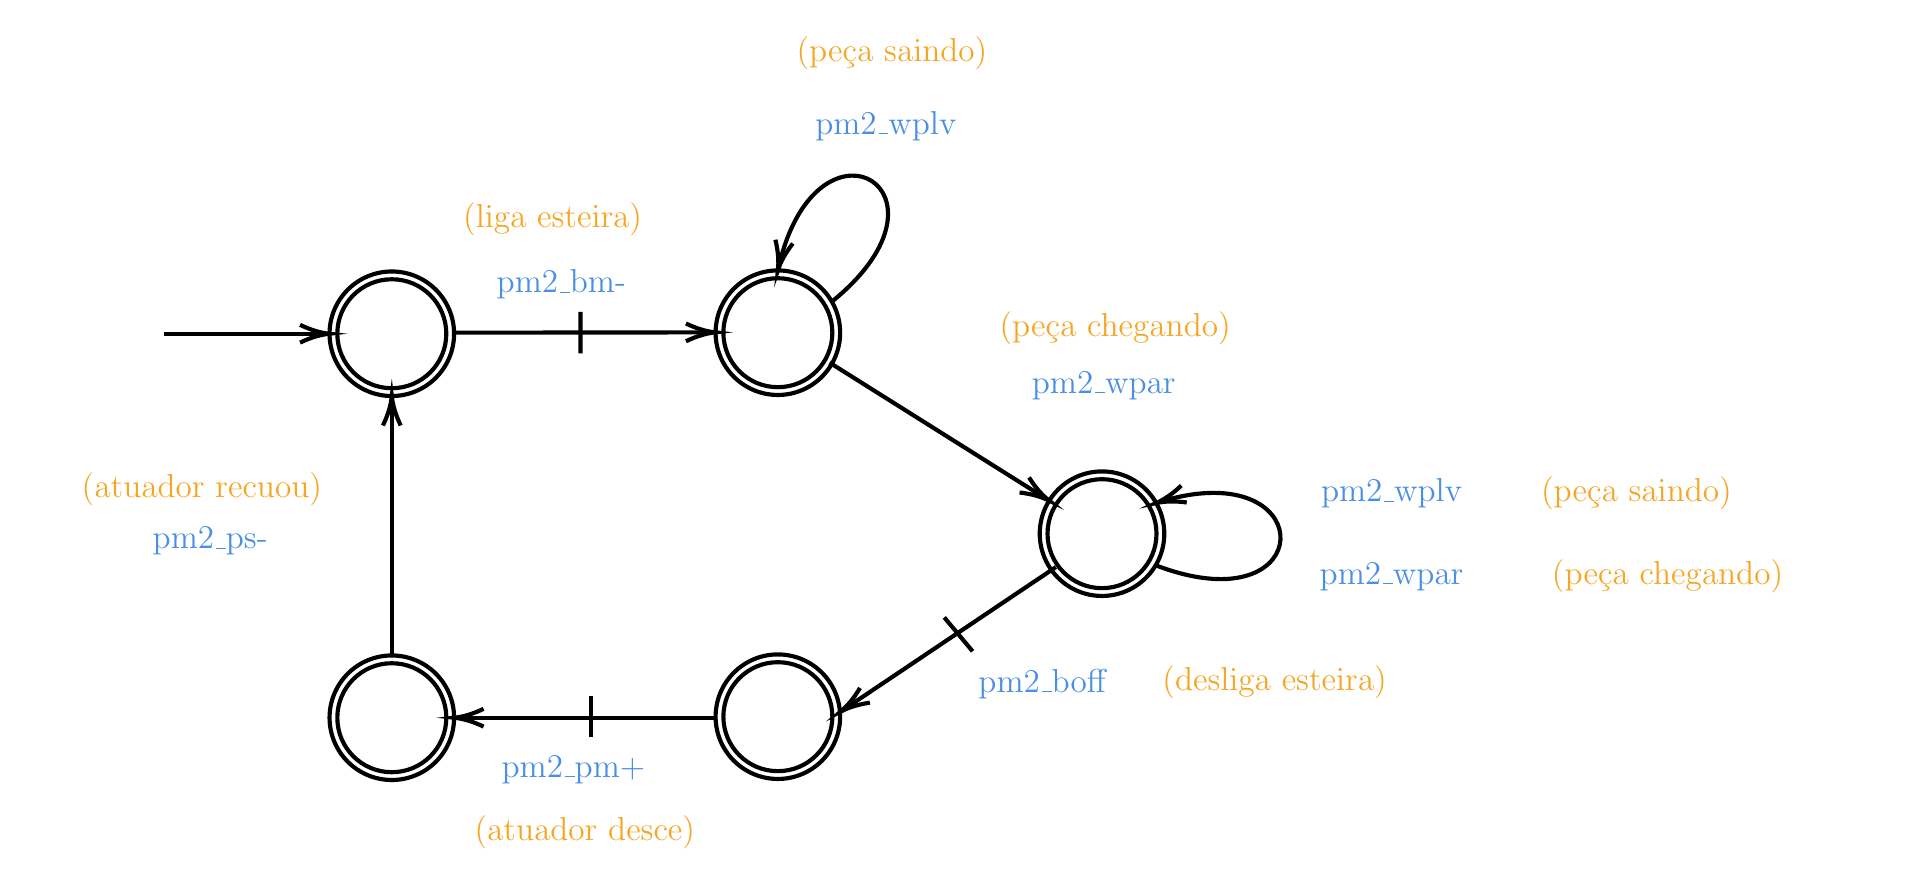
\begin{tikzpicture}[x=0.75pt,y=0.75pt,yscale=-1,xscale=1]
%uncomment if require: \path (0,3420); %set diagram left start at 0, and has height of 3420

%Shape: Circle [id:dp9077579256671899] 
\draw  [line width=1.5]  (1444.5,1540) .. controls (1444.5,1523.43) and (1457.93,1510) .. (1474.5,1510) .. controls (1491.07,1510) and (1504.5,1523.43) .. (1504.5,1540) .. controls (1504.5,1556.57) and (1491.07,1570) .. (1474.5,1570) .. controls (1457.93,1570) and (1444.5,1556.57) .. (1444.5,1540) -- cycle ;
%Shape: Circle [id:dp49050272295100106] 
\draw  [line width=1.5]  (1448.25,1540) .. controls (1448.25,1525.5) and (1460,1513.75) .. (1474.5,1513.75) .. controls (1489,1513.75) and (1500.75,1525.5) .. (1500.75,1540) .. controls (1500.75,1554.5) and (1489,1566.25) .. (1474.5,1566.25) .. controls (1460,1566.25) and (1448.25,1554.5) .. (1448.25,1540) -- cycle ;
%Straight Lines [id:da5069880579739428] 
\draw [line width=1.5]    (1364.5,1540) -- (1441.5,1540) ;
\draw [shift={(1444.5,1540)}, rotate = 180] [color={rgb, 255:red, 0; green, 0; blue, 0 }  ][line width=1.5]    (14.21,-4.28) .. controls (9.04,-1.82) and (4.3,-0.39) .. (0,0) .. controls (4.3,0.39) and (9.04,1.82) .. (14.21,4.28)   ;
%Shape: Circle [id:dp6279882648643924] 
\draw  [line width=1.5]  (1630.5,1539.5) .. controls (1630.5,1522.93) and (1643.93,1509.5) .. (1660.5,1509.5) .. controls (1677.07,1509.5) and (1690.5,1522.93) .. (1690.5,1539.5) .. controls (1690.5,1556.07) and (1677.07,1569.5) .. (1660.5,1569.5) .. controls (1643.93,1569.5) and (1630.5,1556.07) .. (1630.5,1539.5) -- cycle ;
%Straight Lines [id:da9599053460598437] 
\draw [line width=1.5]    (1685.42,1553.91) -- (1704.89,1566.15) -- (1788.71,1618.83) ;
\draw [shift={(1791.25,1620.43)}, rotate = 212.15] [color={rgb, 255:red, 0; green, 0; blue, 0 }  ][line width=1.5]    (14.21,-4.28) .. controls (9.04,-1.82) and (4.3,-0.39) .. (0,0) .. controls (4.3,0.39) and (9.04,1.82) .. (14.21,4.28)   ;
%Straight Lines [id:da49586333480307543] 
\draw [line width=1.5]    (1740.67,1676.67) -- (1754.33,1693) ;
%Shape: Circle [id:dp0045098418455211675] 
\draw  [line width=1.5]  (1630.5,1724.5) .. controls (1630.5,1707.93) and (1643.93,1694.5) .. (1660.5,1694.5) .. controls (1677.07,1694.5) and (1690.5,1707.93) .. (1690.5,1724.5) .. controls (1690.5,1741.07) and (1677.07,1754.5) .. (1660.5,1754.5) .. controls (1643.93,1754.5) and (1630.5,1741.07) .. (1630.5,1724.5) -- cycle ;
%Shape: Circle [id:dp9968433633853042] 
\draw  [line width=1.5]  (1444.5,1725) .. controls (1444.5,1708.43) and (1457.93,1695) .. (1474.5,1695) .. controls (1491.07,1695) and (1504.5,1708.43) .. (1504.5,1725) .. controls (1504.5,1741.57) and (1491.07,1755) .. (1474.5,1755) .. controls (1457.93,1755) and (1444.5,1741.57) .. (1444.5,1725) -- cycle ;
%Straight Lines [id:da3998785728047165] 
\draw [line width=1.5]    (1629.5,1725) -- (1606.5,1725) -- (1507.5,1725) ;
\draw [shift={(1504.5,1725)}, rotate = 360] [color={rgb, 255:red, 0; green, 0; blue, 0 }  ][line width=1.5]    (14.21,-4.28) .. controls (9.04,-1.82) and (4.3,-0.39) .. (0,0) .. controls (4.3,0.39) and (9.04,1.82) .. (14.21,4.28)   ;
%Straight Lines [id:da8755676119075062] 
\draw [line width=1.5]    (1570.5,1734.5) -- (1570.5,1714.5) ;
%Straight Lines [id:da4295420940069248] 
\draw [line width=1.5]    (1474.5,1695) -- (1474.5,1573) ;
\draw [shift={(1474.5,1570)}, rotate = 90] [color={rgb, 255:red, 0; green, 0; blue, 0 }  ][line width=1.5]    (14.21,-4.28) .. controls (9.04,-1.82) and (4.3,-0.39) .. (0,0) .. controls (4.3,0.39) and (9.04,1.82) .. (14.21,4.28)   ;
%Shape: Circle [id:dp9158330958781524] 
\draw  [line width=1.5]  (1634.25,1539.5) .. controls (1634.25,1525) and (1646,1513.25) .. (1660.5,1513.25) .. controls (1675,1513.25) and (1686.75,1525) .. (1686.75,1539.5) .. controls (1686.75,1554) and (1675,1565.75) .. (1660.5,1565.75) .. controls (1646,1565.75) and (1634.25,1554) .. (1634.25,1539.5) -- cycle ;
%Shape: Circle [id:dp9177073337675548] 
\draw  [line width=1.5]  (1448.25,1725) .. controls (1448.25,1710.5) and (1460,1698.75) .. (1474.5,1698.75) .. controls (1489,1698.75) and (1500.75,1710.5) .. (1500.75,1725) .. controls (1500.75,1739.5) and (1489,1751.25) .. (1474.5,1751.25) .. controls (1460,1751.25) and (1448.25,1739.5) .. (1448.25,1725) -- cycle ;
%Shape: Circle [id:dp13905839114905638] 
\draw  [line width=1.5]  (1634.25,1724.5) .. controls (1634.25,1710) and (1646,1698.25) .. (1660.5,1698.25) .. controls (1675,1698.25) and (1686.75,1710) .. (1686.75,1724.5) .. controls (1686.75,1739) and (1675,1750.75) .. (1660.5,1750.75) .. controls (1646,1750.75) and (1634.25,1739) .. (1634.25,1724.5) -- cycle ;
%Shape: Circle [id:dp5145905470381016] 
\draw  [line width=1.5]  (1786.67,1636.33) .. controls (1786.67,1619.76) and (1800.1,1606.33) .. (1816.67,1606.33) .. controls (1833.24,1606.33) and (1846.67,1619.76) .. (1846.67,1636.33) .. controls (1846.67,1652.9) and (1833.24,1666.33) .. (1816.67,1666.33) .. controls (1800.1,1666.33) and (1786.67,1652.9) .. (1786.67,1636.33) -- cycle ;
%Shape: Circle [id:dp43990026803091764] 
\draw  [line width=1.5]  (1790.42,1636.33) .. controls (1790.42,1621.84) and (1802.17,1610.08) .. (1816.67,1610.08) .. controls (1831.16,1610.08) and (1842.92,1621.84) .. (1842.92,1636.33) .. controls (1842.92,1650.83) and (1831.16,1662.58) .. (1816.67,1662.58) .. controls (1802.17,1662.58) and (1790.42,1650.83) .. (1790.42,1636.33) -- cycle ;
%Shape: Boxed Bezier Curve [id:dp1547709151209966] 
\draw [line width=1.5]    (1686.43,1524.6) .. controls (1747.82,1475.02) and (1689.13,1434.17) .. (1665.64,1492.43) .. controls (1663.94,1496.64) and (1662.42,1501.37) .. (1661.15,1506.65) ;
\draw [shift={(1660.5,1509.5)}, rotate = 282.21] [color={rgb, 255:red, 0; green, 0; blue, 0 }  ][line width=1.5]    (14.21,-4.28) .. controls (9.04,-1.82) and (4.3,-0.39) .. (0,0) .. controls (4.3,0.39) and (9.04,1.82) .. (14.21,4.28)   ;
%Shape: Boxed Line [id:dp94520568482204] 
\draw [line width=1.5]    (1794.44,1652.44) -- (1693.15,1720.45) ;
\draw [shift={(1690.66,1722.12)}, rotate = 326.12] [color={rgb, 255:red, 0; green, 0; blue, 0 }  ][line width=1.5]    (14.21,-4.28) .. controls (9.04,-1.82) and (4.3,-0.39) .. (0,0) .. controls (4.3,0.39) and (9.04,1.82) .. (14.21,4.28)   ;
%Shape: Boxed Bezier Curve [id:dp2849664697222474] 
\draw [line width=1.5]    (1842.67,1651.61) .. controls (1916.4,1679.72) and (1922.18,1608.45) .. (1860,1617.46) .. controls (1855.51,1618.11) and (1850.66,1619.18) .. (1845.46,1620.74) ;
\draw [shift={(1842.67,1621.61)}, rotate = 342] [color={rgb, 255:red, 0; green, 0; blue, 0 }  ][line width=1.5]    (14.21,-4.28) .. controls (9.04,-1.82) and (4.3,-0.39) .. (0,0) .. controls (4.3,0.39) and (9.04,1.82) .. (14.21,4.28)   ;
%Straight Lines [id:da30354536494497486] 
\draw [line width=1.5]    (1505.42,1539.48) -- (1528.42,1539.46) -- (1627.42,1539.34) ;
\draw [shift={(1630.42,1539.33)}, rotate = 179.93] [color={rgb, 255:red, 0; green, 0; blue, 0 }  ][line width=1.5]    (14.21,-4.28) .. controls (9.04,-1.82) and (4.3,-0.39) .. (0,0) .. controls (4.3,0.39) and (9.04,1.82) .. (14.21,4.28)   ;
%Straight Lines [id:da805241114651789] 
\draw [line width=1.5]    (1565.4,1529.41) -- (1565.43,1549.41) ;


% Text Node
\draw (1556.17,1516.33) node  [font=\large] [align=left] {\begin{minipage}[lt]{58.23pt}\setlength\topsep{0pt}
\begin{center}
\textcolor[rgb]{0.29,0.56,0.89}{pm2\_bm-}
\end{center}

\end{minipage}};
% Text Node
\draw (1552,1485) node  [font=\large] [align=left] {\begin{minipage}[lt]{119.21pt}\setlength\topsep{0pt}
\begin{center}
\textcolor[rgb]{0.96,0.65,0.14}{(liga esteira)}
\end{center}

\end{minipage}};
% Text Node
\draw (1562,1750) node  [font=\large] [align=left] {\begin{minipage}[lt]{57.55pt}\setlength\topsep{0pt}
\begin{center}
\textcolor[rgb]{0.29,0.56,0.89}{pm2\_pm+}
\end{center}

\end{minipage}};
% Text Node
\draw (1567.5,1780) node  [font=\large] [align=left] {\begin{minipage}[lt]{112.65pt}\setlength\topsep{0pt}
\begin{center}
\textcolor[rgb]{0.96,0.65,0.14}{(atuador desce)}
\end{center}

\end{minipage}};
% Text Node
\draw (1387,1640) node  [font=\large] [align=left] {\begin{minipage}[lt]{57.55pt}\setlength\topsep{0pt}
\begin{center}
\textcolor[rgb]{0.29,0.56,0.89}{pm2\_ps-}
\end{center}

\end{minipage}};
% Text Node
\draw (1383,1615) node  [font=\large] [align=left] {\begin{minipage}[lt]{119.22pt}\setlength\topsep{0pt}
\begin{center}
\textcolor[rgb]{0.96,0.65,0.14}{(atuador recuou)}
\end{center}

\end{minipage}};
% Text Node
\draw (1712.5,1440) node  [font=\large] [align=left] {\begin{minipage}[lt]{58.23pt}\setlength\topsep{0pt}
\begin{center}
\textcolor[rgb]{0.29,0.56,0.89}{pm2\_wplv}
\end{center}

\end{minipage}};
% Text Node
\draw (1715.5,1405) node  [font=\large] [align=left] {\begin{minipage}[lt]{156.17pt}\setlength\topsep{0pt}
\begin{center}
\textcolor[rgb]{0.96,0.65,0.14}{(peça saindo)}
\end{center}

\end{minipage}};
% Text Node
\draw (1817.5,1565) node  [font=\large] [align=left] {\begin{minipage}[lt]{58.23pt}\setlength\topsep{0pt}
\begin{center}
\textcolor[rgb]{0.29,0.56,0.89}{pm2\_wpar}
\end{center}

\end{minipage}};
% Text Node
\draw (1823.01,1537.33) node  [font=\large] [align=left] {\begin{minipage}[lt]{143.25pt}\setlength\topsep{0pt}
\begin{center}
\textcolor[rgb]{0.96,0.65,0.14}{(peça chegando)}
\end{center}

\end{minipage}};
% Text Node
\draw (1787.83,1708.67) node  [font=\large] [align=left] {\begin{minipage}[lt]{58.23pt}\setlength\topsep{0pt}
\begin{center}
\textcolor[rgb]{0.29,0.56,0.89}{pm2\_boff}
\end{center}

\end{minipage}};
% Text Node
\draw (1899.83,1707.67) node  [font=\large] [align=left] {\begin{minipage}[lt]{156.17pt}\setlength\topsep{0pt}
\begin{center}
\textcolor[rgb]{0.96,0.65,0.14}{(desliga esteira)}
\end{center}

\end{minipage}};
% Text Node
\draw (1956.17,1657) node  [font=\large] [align=left] {\begin{minipage}[lt]{58.23pt}\setlength\topsep{0pt}
\begin{center}
\textcolor[rgb]{0.29,0.56,0.89}{pm2\_wpar}
\end{center}

\end{minipage}};
% Text Node
\draw (2089.17,1657) node  [font=\large] [align=left] {\begin{minipage}[lt]{156.17pt}\setlength\topsep{0pt}
\begin{center}
\textcolor[rgb]{0.96,0.65,0.14}{(peça chegando)}
\end{center}

\end{minipage}};
% Text Node
\draw (1956.17,1617) node  [font=\large] [align=left] {\begin{minipage}[lt]{58.23pt}\setlength\topsep{0pt}
\begin{center}
\textcolor[rgb]{0.29,0.56,0.89}{pm2\_wplv}
\end{center}

\end{minipage}};
% Text Node
\draw (2074.17,1617) node  [font=\large] [align=left] {\begin{minipage}[lt]{156.17pt}\setlength\topsep{0pt}
\begin{center}
\textcolor[rgb]{0.96,0.65,0.14}{(peça saindo)}
\end{center}

\end{minipage}};


\end{tikzpicture}